\authoredsubsection{Sprint 4}{Mohsin}{Mohsin Saeed}\label{sec:sprint4}

Sprint 4 ran from 10 to 23 June 2026, with the review on 24 June, and marked the transition from independently functioning components to a unified system. By the end of Sprint 3 the router, judge, and optimizer each worked on their own but still communicated through direct subprocess calls and local JSON files, so any change to one module risked breaking the others. Sprint 4 set out to replace that fragile arrangement with an integrated, end-to-end pipeline that could be run, observed, and evaluated as one system. Mohsin Saeed served as the Scrum Master for this sprint.

\subsubsection{Sprint Goals}\label{sec:sprint4-goals}

The sprint goal was to deliver a complete, end-to-end pipeline that a user could run as a unified system, resting on three deliverables: a centralized pipeline skeleton that formally defined the interfaces between all components through a single orchestration layer, a finalized decision between the OPRO and DSPy optimizers together with its integration, and a pipeline visualization dashboard that made every routing and evaluation step inspectable in real time. The goal met the SMART criteria, with a measurable outcome in that a user could submit a query and inspect the full loop, and was time-bound to the two-week sprint ending 23 June 2026 \autocite{schwaber2020scrum}.

\subsubsection{Sprint Planning}\label{sec:sprint4-planning}

The direction had been set at the Sprint 3 review, where Interhyp's product owners, Julian Kappler and Rainer Bomblies, described Sprint 4 as the decisive test of the integrated architecture. The team had already identified the need for an orchestration layer to replace the direct calls between modules. The backlog held seven tickets totaling 25 story points, consistent with prior velocity, but was structured differently (\cref{fig:sprint4-backlog}): the two highest-weight tickets, the pipeline skeleton and the dashboard at eight points each, were treated as shared team efforts spanning the Python worker, the Convex backend, and the React frontend, reflecting how much coordination integration work would demand.

\begin{figure}
\centering
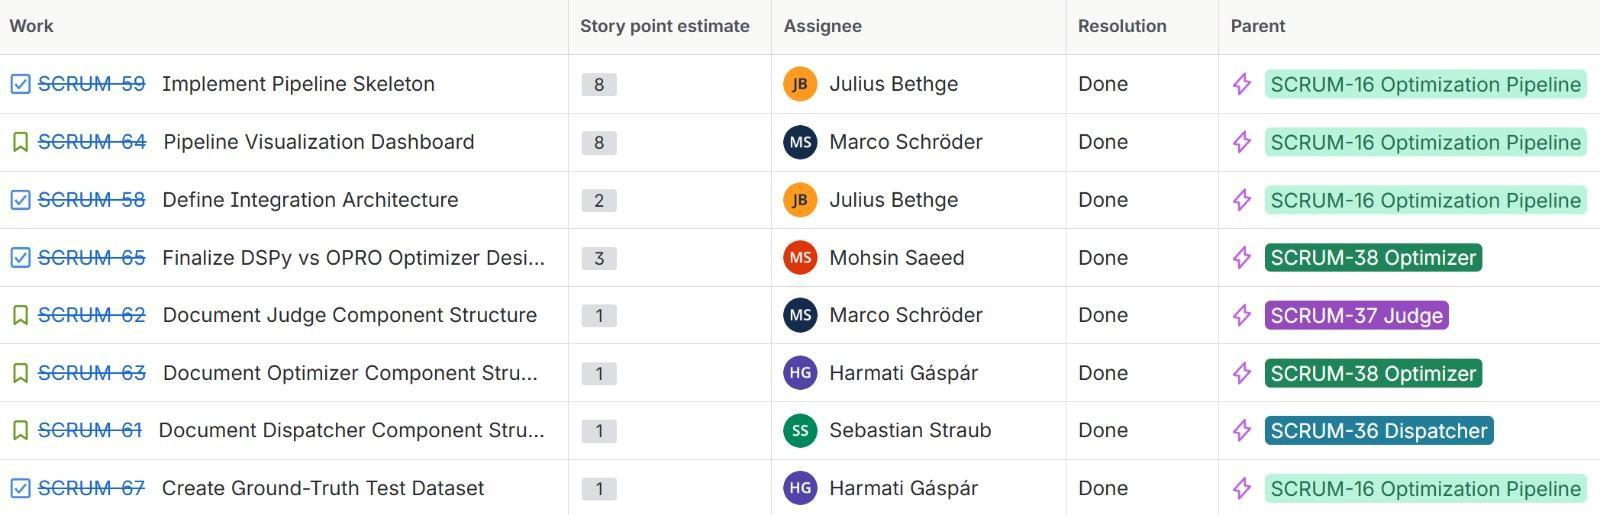
\includegraphics[width=1\linewidth,height=\textheight,keepaspectratio]{assets/sprints/sprint4-backlog.jpg}
\caption{Sprint 4 backlog in Jira, showing the seven tickets and their story-point weights.}\label{fig:sprint4-backlog}
\end{figure}

\subsubsection{Implementation and Execution}\label{sec:sprint4-implementation}

Execution began before any integration code was written, with each module owner documenting their own component on a shared document, so that every member started with a clear picture of the others' modules rather than relying on the ad-hoc explanations that had slowed earlier sprints. During a dedicated design session, the team defined an architecture with three runtime processes: the React frontend renders the UI, Convex manages application state and job scheduling, and the Python worker executes all pipeline logic. Routing all communication through Convex decoupled the components, eliminating the fragility of the Sprint 3 design. Convex was chosen for its real-time streaming, its native vector search on which Stage 1 depends, its typed schema, and its local and hosted deployment support.

On this foundation the team implemented the pipeline skeleton. A Python worker continuously polls Convex, claims the oldest queued job, and executes it across four job types: a chat run, a judge evaluation, a batch run against a labeled dataset, and an optimization run over accumulated judge feedback. Each job maps to a fixed sequence of named steps recorded in Convex, so the frontend always shows what happened, including branches skipped when Stage 1 routed a query directly.

Stage 1 was rebuilt on Convex's vector search: a query is embedded with FastEmbed's multilingual-e5-large model, its nearest neighbors are grouped by agent, and the margin between the top two is compared against a per-agent threshold, with Stage 2 calling Ollama and selecting the agent with the highest log-probability only if the margin is not met. New vector entries are held in memory throughout a batch run and inserted only after every row is processed, preventing leakage within a batch and addressing a risk Julian had raised in Sprint 3.

In parallel, the team also built the pipeline visualization dashboard in React on Convex subscriptions, so the interface updates live. The chat view shows the selected agent, the routing stage, and the confidence scores behind a decision (\cref{fig:sprint4-chat-view}), while the pipeline view renders the router and judge flows as interactive diagrams whose highlighted path shows which branches executed (\cref{fig:sprint4-router-pipeline}).

\begin{figure}
\centering
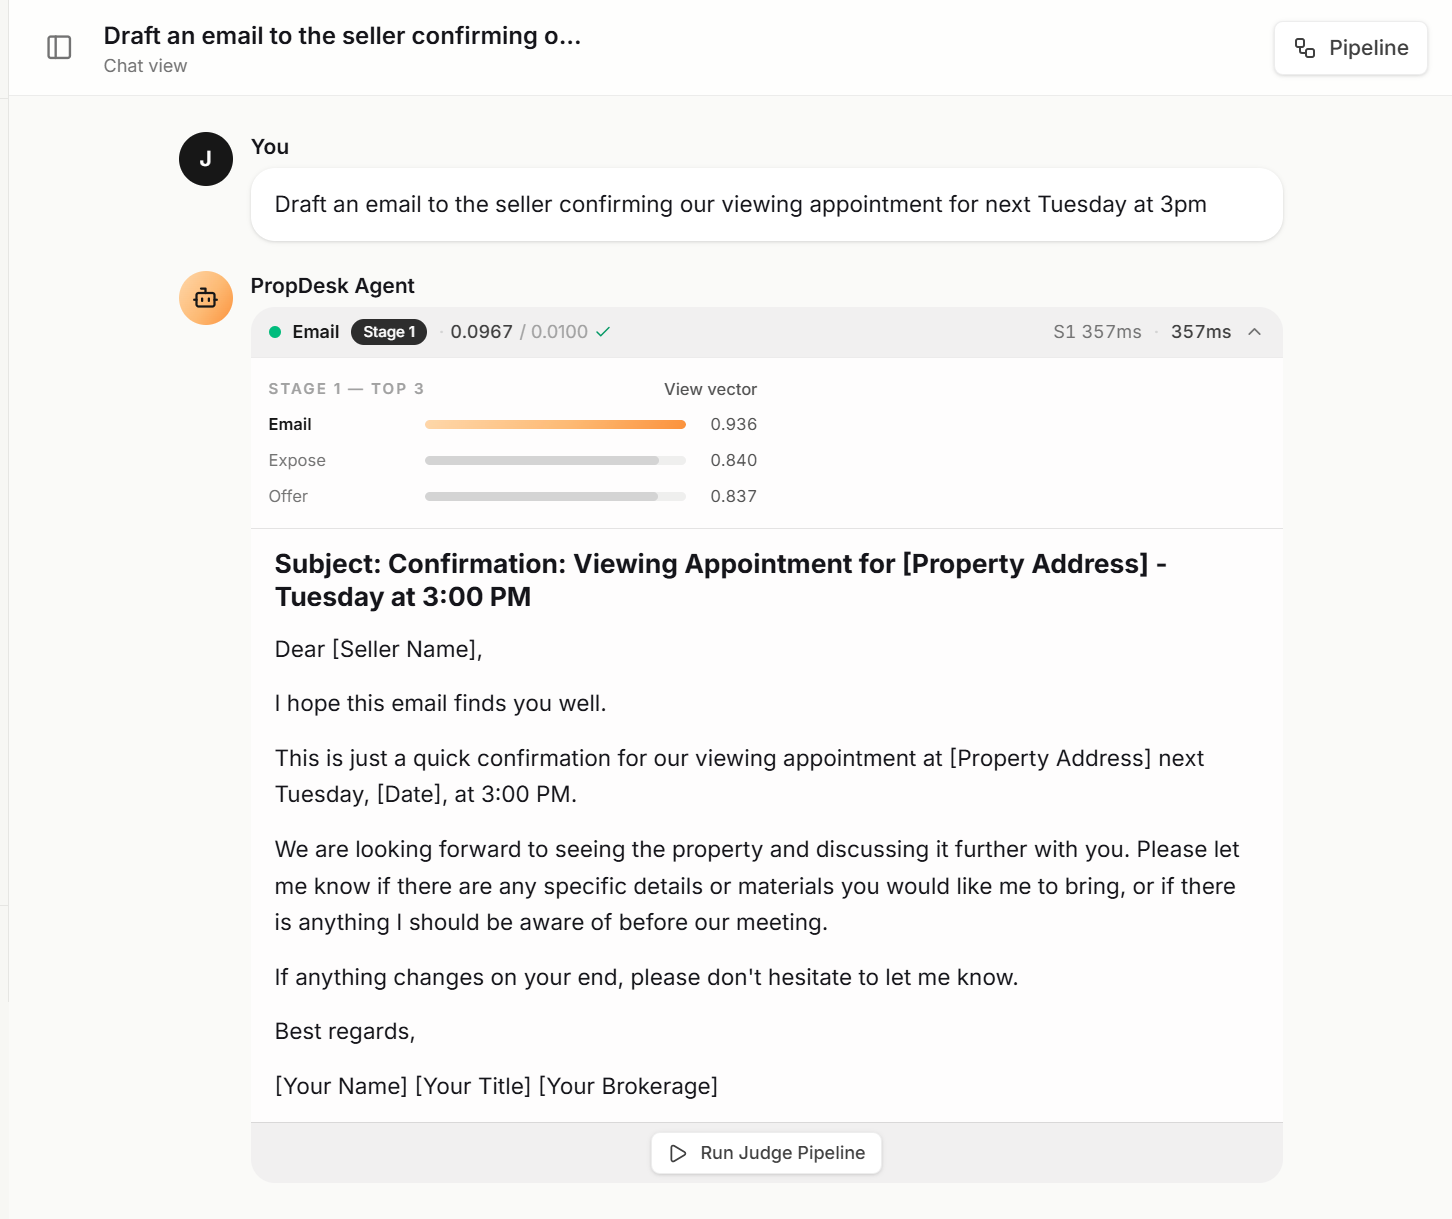
\includegraphics[width=0.7\linewidth,height=\textheight,keepaspectratio]{assets/sprints/sprint4-chat-view.png}
\caption{Chat view showing the routed agent, the Stage 1 routing decision, and the per-agent confidence scores.}\label{fig:sprint4-chat-view}
\end{figure}

\begin{figure}
\centering
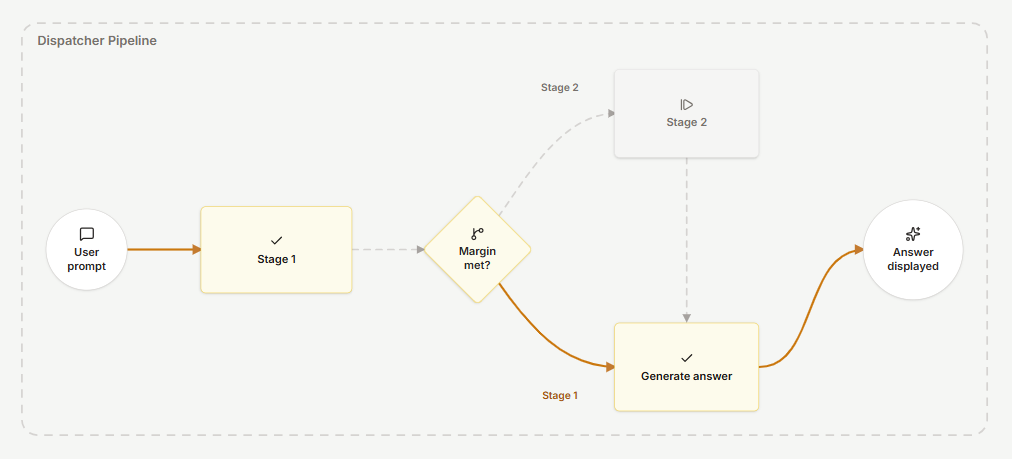
\includegraphics[width=1\linewidth,height=\textheight,keepaspectratio]{assets/sprints/sprint4-router-pipeline.png}
\caption{Router pipeline diagram, with the highlighted path showing a query routed directly by Stage 1 and Stage 2 left skipped.}\label{fig:sprint4-router-pipeline}
\end{figure}

The remaining architectural decision was the choice of optimizer. On a shared 548-example set covering all eight agents, DSPy MIPROv2 improved Stage 2 accuracy from 95.45 to 96.59 percent, a gain of 1.14 percentage points, but only once the dataset was large enough to expose a consistent signal. On the same data, OPRO reached 98.6 percent from a comparable baseline in six rounds. The difference lies in the optimization strategy: rather than searching statistically over a validation set, OPRO grounds its meta-prompt in judge-confirmed routing failures, refining the prompt from explicit failure cases instead of requiring broad coverage of the task distribution \autocite{yang2023llmoptimizers}. The team selected OPRO and aligned the decision with Julian and Rainer on 16 June. To measure improvement without bias, Gáspár then built a deliberately difficult ground-truth test dataset across all eight agents, held out from every optimization run.

\subsubsection{Sprint Review}\label{sec:sprint4-review}

The review took place on 23 June 2026 over Microsoft Teams with Julian and Rainer. After presenting the OPRO decision, the team ran the full pipeline end to end, from a query through routing and response to a judge evaluation. The highlight was a live demonstration of the self-improvement loop: because the judge had written new vector entries during the demo, the product owners asked whether a query that had previously required Stage 2 would now be handled by Stage 1 directly. It was, confirming in real time that the judge's corrections were improving routing. Julian raised a concern about the Stage 1 vector index growing over time, and the team pointed to the novelty check that prevents near-duplicate entries and proposed approximate nearest-neighbor search for scale. Both product owners gave their strongest endorsement so far, noting that the team now had a product worth presenting to a wider audience and advising it to step back in the final sprint to communicate what had been built rather than adding features.

The team completed all seven user stories and delivered the full 25 story points. The burndown (\cref{fig:sprint4-burndown}) stayed flat for much of the sprint and dropped sharply near the end, reflecting the nature of the integration work. The two largest tickets, the skeleton and dashboard, could only be closed once fully completed.

\begin{figure}
\centering
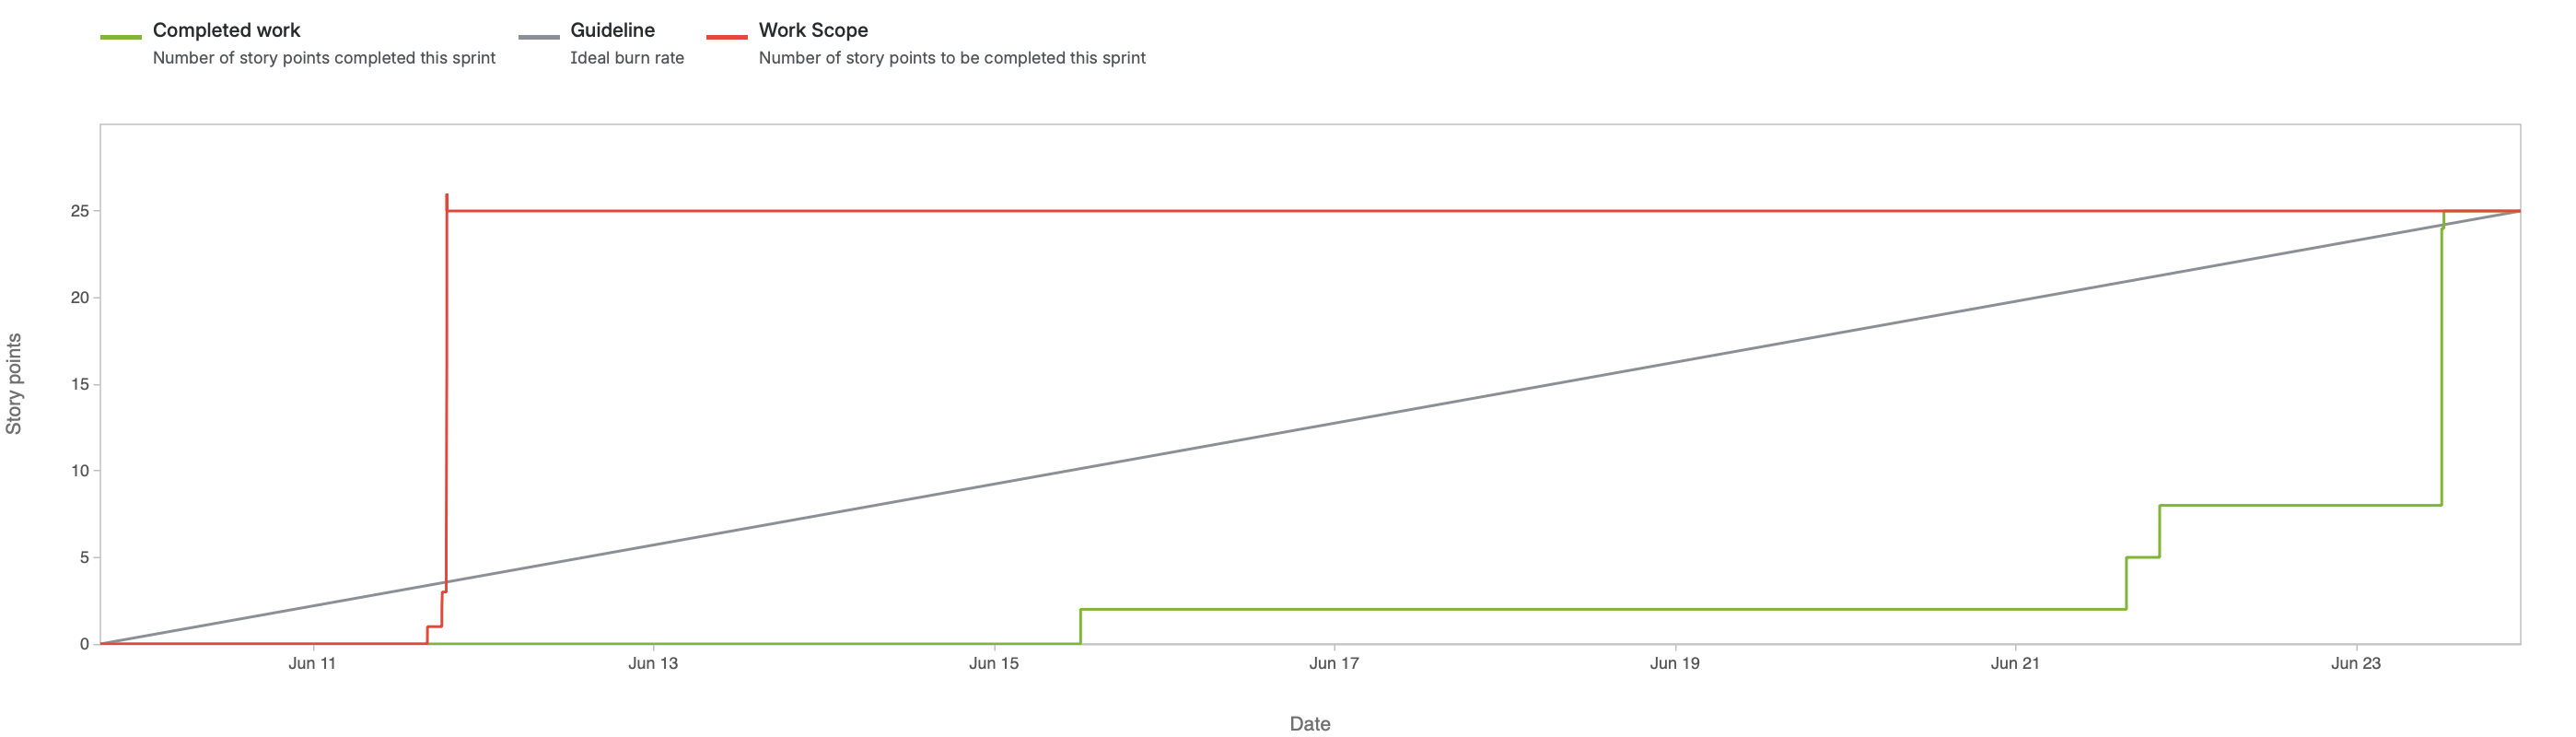
\includegraphics[width=1\linewidth,height=\textheight,keepaspectratio]{assets/sprints/sprint4-burndown.png}
\caption{Sprint 4 burndown chart, flat through the sprint and dropping as the two large integration tickets closed.}\label{fig:sprint4-burndown}
\end{figure}

\subsubsection{Sprint Retrospective}\label{sec:sprint4-retrospective}

The Sprint 4 retrospective used an adapted Sailboat format (\cref{fig:sprint4-sailboat}), based on a publicly available Miro template \autocite{miro2024sailboat}, chosen to keep the session engaging and frame the sprint within the wider project. Held on 23 June within a strict forty-minute timebox, it moved through four themes. Under Tailwinds the team credited coordination, planning together before building, and the increased meeting cadence. The Delights centered on the product finally feeling complete and ready to demonstrate, with the dashboard and the clarity of the optimizer decision singled out. The Restraints were personal rather than technical, dominated by exams and university stress, while the absence of any technical blocker was itself a signal that earlier integration friction had been resolved. The Future Risks looked ahead to the exam period as a capacity risk and to the challenge of making a complex product understandable to a broader audience, a shift from solving technical integration problems toward managing delivery risk and communication as the project approached completion.

\begin{figure}
\centering
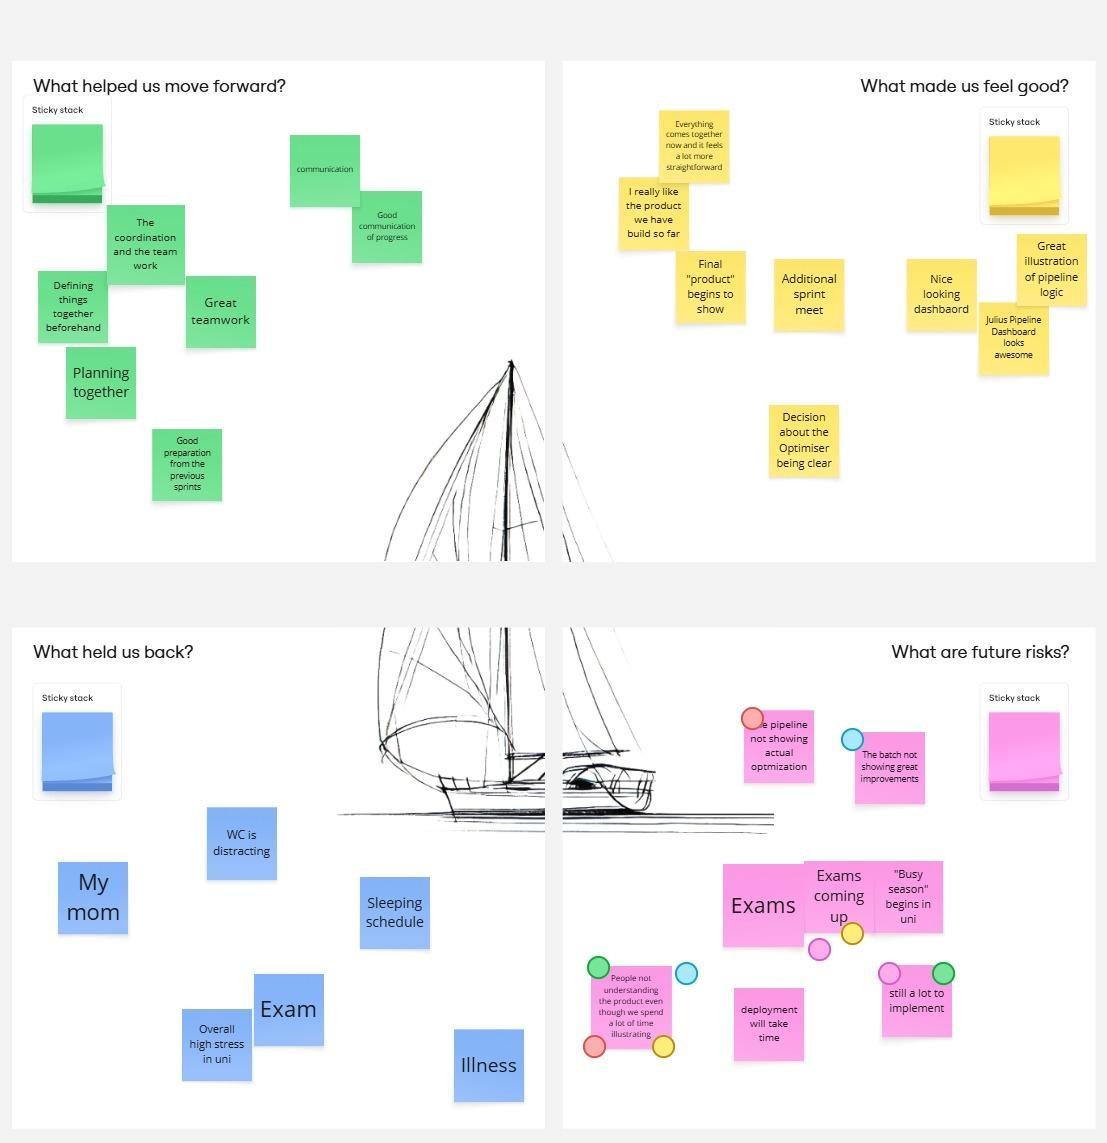
\includegraphics[width=0.65\linewidth,height=\textheight,keepaspectratio]{assets/sprints/sprint4-retrospective.jpg}
\caption{Sailboat retrospective board, with Tailwinds and Delights on the top row and Restraints and Future Risks below.}\label{fig:sprint4-sailboat}
\end{figure}

Two action items were adopted for Sprint 5. First, each member would block dedicated time around the exam period to protect the team's capacity for the final sprint, directly addressing the risk that had dominated the retrospective. Second, the team committed to delivering a well-defined dashboard by 30 June, the technical priority flagged as still outstanding. Both were assigned to the team as a whole rather than to individual owners, reflecting the collaborative nature of the final stretch (\cref{fig:sprint4-action-items}).

\begin{figure}
\centering
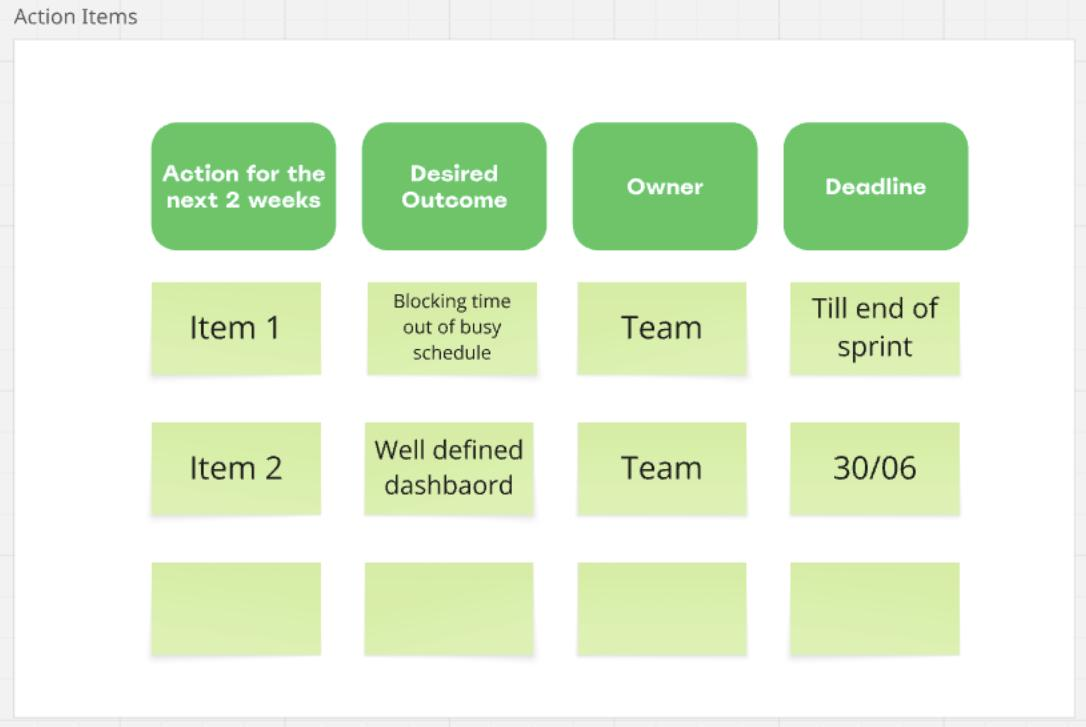
\includegraphics[width=1\linewidth,height=\textheight,keepaspectratio]{assets/sprints/sprint4-action-items.jpg}
\caption{The two action items agreed in the retrospective for Sprint 5: protecting team capacity during the exam period and delivering a well-defined dashboard by 30 June.}\label{fig:sprint4-action-items}
\end{figure}
